\section{Пример использования}

Рассмотрим пример для обработки данных по численности постоянного населения Москвы и Санкт-Петербурга за период 2000-2021 годов.

Наши данные выглядят следующим образом:

\begin{figure}[H]
	\begin{center}
		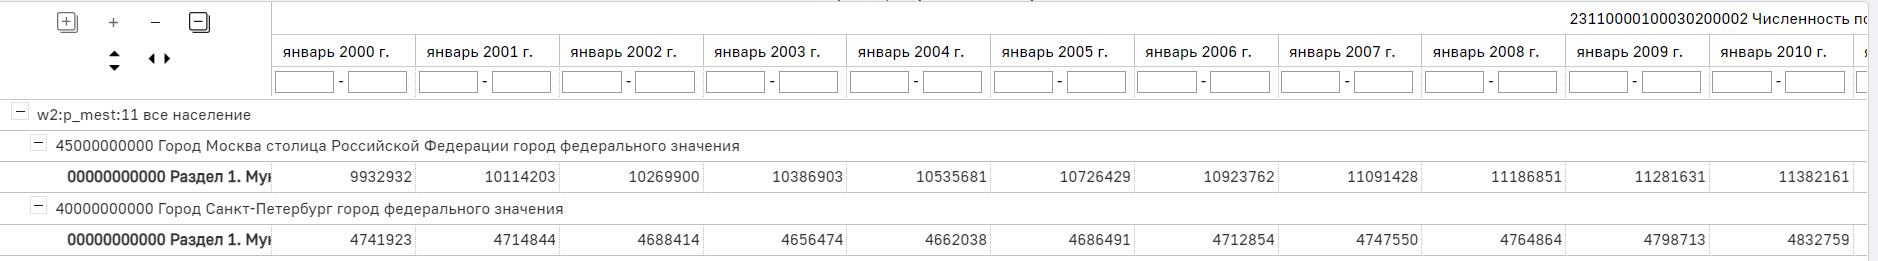
\includegraphics[scale = 0.47]{include/fig/data_rosstat}
	\end{center}
\end{figure}

Всего
\href{https://showdata.gks.ru/finder/descriptors/278928}{Росстат} выделяет нам 6 строчек, из которых нужные нам -- 4ая и 6ая.

Открываем Pycharm (Visual Studio Code) и создаем .py-файл. Перво-наперво подключаем нужные нам библиотеки и модули при помощи функции \textit{import}:

\begin{figure}[H]
	\begin{center}
		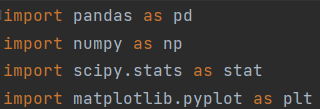
\includegraphics{include/fig/import}
	\end{center}
\end{figure}

Pandas нужен для чтения .xlsx-файла и дальнешей работы с данными; Numpy -- для работы с массивами и вычислениями основным статистик; модуль stats из библиотеки Scipy позволяет вычислять некоторые иными статистики, которых нет в Numpy; и, наконец, модуль pyplot для рисования графиков. Приписка \textit{... as ...} в каждой строчке упрощает обращение к библиотекам -- теперь нет необходимости писать её длинное название, достаточно лишь написать сокращение, которое мы сами можем выбрать.

Далее следует скачать таблицу и поместить её в одну папку с .py-файлом. Для простоты я переименовал её в "moscow\_spb.xlsx". Таким образом, воспользуемся функцией из Pandas для чтения .xlsx-файла:

\begin{figure}[H]
	\begin{center}
		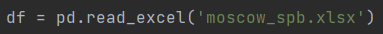
\includegraphics{include/fig/readexcel}
	\end{center}
\end{figure}

Теперь мы можем посмотреть, что внутри переменной df.

\begin{figure}[H]
	\begin{center}
		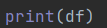
\includegraphics{include/fig/printdf}
	\end{center}
\end{figure}

И мы получим:

\begin{figure}[H]
	\begin{center}
		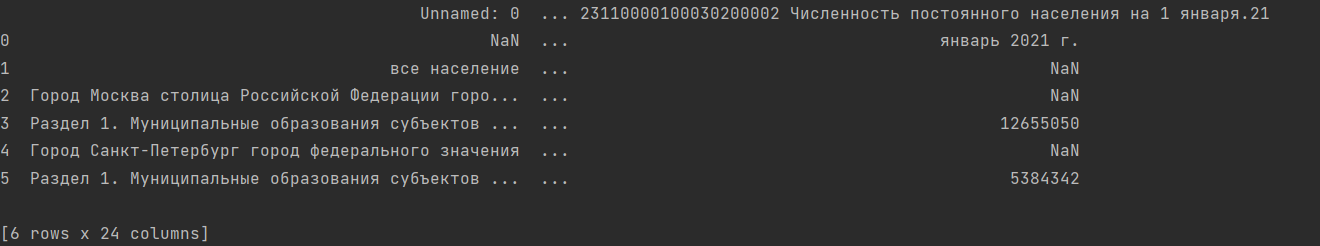
\includegraphics[scale=0.65]{include/fig/print}
	\end{center}
\end{figure}

Да, он не вывел нам всю таблицу, но можно увидеть, что сейчас в датафрейме 6 строк и 24 колонки. Изначально мы уже определили, что нам нужно 2 строчки, а период с 2000 по 2021 составляет 22 значения. Соответственно, нам необходимо "почистить" эти данные.

Со строчками мы определились выше -- 4ая и 6ая, а с колонками всё иначе. Первые две колонки содержат ненужные индексы, а их названия слишком громоздки. Программно это выглядит следующим образом:

\begin{figure}[H]
	\begin{center}
		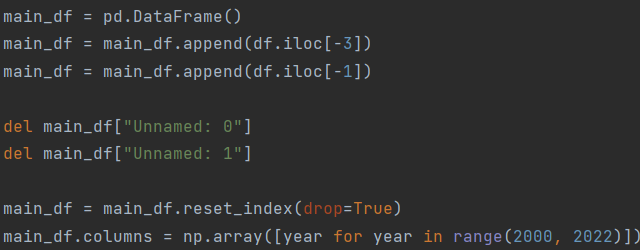
\includegraphics{include/fig/maindf}
	\end{center}
\end{figure}

Сначала мы создаем пустой датафрейм, куда мы положим нужные нам столбцы и строки. Затем мы добавляем нужную строку при помощи метода .append. То, что находится в скобках после .append -- это то, что мы добавляем в main\_df. Метод .iloc позволяет обращаться к строкам датафрейма по индексу. Этот индекс начинается с нуля, то есть, df.iloc[0] выдаст нам первую строчку, df.iloc[1] -- вторую и т.д.. Однако массивы в Python позволяют принимать отрицательные значения, что равносильно "проходу по массиву" в обратную сторону. Это значит, что df.iloc[-1] выдаст последнюю строку, а df.iloc[-3] - третью с конца. Итак, строки добавлены.

Далее мы определили, что первые две колонки содержат незначащие индексы и подписи, поэтому при помощи функции del эти колонки последовательно удаляются. Так как у них не было названия, к ним можно обратиться как "Unnamed: 0" и "Unnamed: 1" соответственно.

Если мы посмотрим на наш датафрейм сейчас, то увидим громоздкие названия столбцов и неверые индексы у строк. К названиям столбцов можно обратиться при помощи метода .columns, а присвоение чего-либо соизмеримого их просто переименует. Так показано, что мы добавляем массив (array), в котором последовательно указаны все года (все целые значения), принадлежащие полуинтервалу $\left[2000, 2022\right)$. У любого датафрейма также есть возможность сбросить по умолчанию нумерацию строк -- .reset\_index(drop=True).

"Очищенные" данные выглядят следующим образом:

\begin{figure}[H]
	\begin{center}
		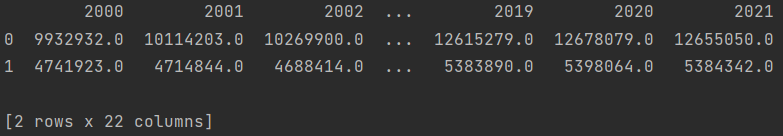
\includegraphics{include/fig/cleardf}
	\end{center}
\end{figure}

Первый город -- Москва, второй -- Санкт-Петербург. То есть, наша задача сводится к тому, чтобы пройти датафрейм построчно, описать данные и нанести их на график.

Метод .iterrows() выдает нам 2 значения -- индекс строки и саму строку. Таким образом, запустив цикл, мы можем "пройтись" по всем строкам. То есть,

\begin{figure}[H]
	\begin{center}
		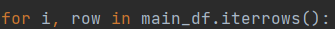
\includegraphics{include/fig/iterrows}
	\end{center}
\end{figure}

На каждой из двух итераций в переменную row будет записан массив с 22мя значениями. Этого хватит, чтобы найти разные статистики.

\begin{figure}[H]
	\begin{center}
		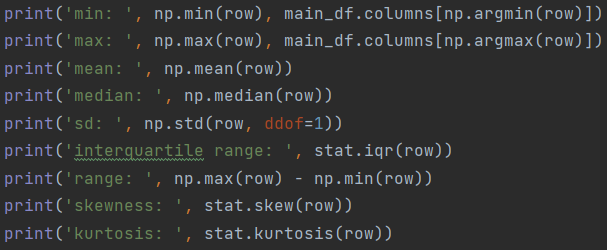
\includegraphics{include/fig/describe}
	\end{center}
\end{figure}

По порядку:
\begin{itemize}
	\item min - минимум;
	\item max - максимум;
	\item mean - среднее;
	\item median - медиана;
	\item sd (std) - стандартное отклонение;
	\item interquartile range (iqr) - интерквартильный размах;
	\item range - размах;
	\item skewness (skew) - коэффициент асимметрии;
	\item kurtosis - эксцесс.
\end{itemize}

\newpage

